% http://www.idsc.ethz.ch/education/theses-semester-projects.html
% IDSC LaTeX Thesis Template
% 
% Author(s):	Eric Müller
% 				Institute for Dynamic Systems and Control
% 				Swiss Federal Institute of Technology (ETH) Zurich
% 
% Created:		2004/04/02  (Eric Mueller)
% 
% Notes: Has been tested on Windows 7 + MikTeX + TeXnicCenter
%
% Revisions: 	2009/05/29  (Soren Ebbesen)
% 				    2011/03/22	(Soren Ebbesen)
%             2013/03/08	(Soren Ebbesen)
%             2014/03/13	(Soren Ebbesen)
% ______________________________________________________________________________
\documentclass[10pt,twoside,a4paper,fleqn]{report}


\usepackage[english,st]{ethidsc} % Special IDSC styles and commands      	
								 % {german}/english: language of headings, etc.
								 % {st}/bt/mt: {semester}/bachelor/master thesis
							
% Page header (don't change)____________________________________________________
\setlength{\parindent}{0em}                 % Disable parindent
\rhead[\nouppercase{\rightmark}]{\thepage}  % Special headings
\lhead[\thepage]{\nouppercase{\leftmark}}   % Special headings
\cfoot{}                                    % Special headings


% Title page (please fill in)___________________________________________________
\title{\LaTeX\ Thesis Template v.1.4}


\studentA{Hans Muster}
\ethidA{97-906-739}
\semesterA{5}
\emailA{muster@student.ethz.ch}

%\studentB{Second Student}
%\ethidB{12-345-678}
%\semesterB{9}
%\emailB{second@student.ethz.ch}

\supervision{First Supervisor\\ Prof. Dr. Second Supervisor}
\date{March 2011}

\identification{IDSC-XX-YY-ZZ} 		% Project identifier

\infopage
\declaration

% Begin document________________________________________________________________
\begin{document}

\maketitle 							% Create title page


% Preamble______________________________________________________________________

\pagenumbering{roman} 				% Begin roman page numbering (i,ii,...)

%---------------------------------------------------------------------------
% Preface

\chapter*{Preface}

Blah blah \dots

 \cleardoublepage

%---------------------------------------------------------------------------
% Table of contents

 \setcounter{tocdepth}{2}
 \tableofcontents

 \cleardoublepage

%---------------------------------------------------------------------------
% Abstract

\chapter*{Zusammenfassung}
 \addcontentsline{toc}{chapter}{Zusammenfassung}

Bla bla \dots

 \cleardoublepage

\chapter*{Abstract}
 \addcontentsline{toc}{chapter}{Abstract}

Blah blah \dots

 \cleardoublepage

%---------------------------------------------------------------------------
% Symbols

\chapter*{Nomenclature}\label{chap:symbole}
 \addcontentsline{toc}{chapter}{Nomenclature}

\section*{Symbols}
\begin{tabbing}
 \hspace*{1.6cm} \= \hspace*{8cm} \= \kill
 $\mathrm{EHC}$ \> Conditional equation \> [$-$] \\[0.5ex]
 $e$ \> Willans coefficient \> [$-$] \\[0.5ex]
 $F,G$ \> Parts of the system equation \> [\unitfrac[]{K}{s}]
\end{tabbing}

\section*{Indicies}
\begin{tabbing}
 \hspace*{1.6cm}  \= \kill
 a \> Ambient \\[0.5ex]
 air \> Air
\end{tabbing}

\section*{Acronyms and Abbreviations}
\begin{tabbing}
 \hspace*{1.6cm}  \= \kill
 NEDC \> New European Driving Cycle \\[0.5ex]
 ETH \> Eidgen\"{o}ssische Technische Hochschule
\end{tabbing}

 \cleardoublepage

%---------------------------------------------------------------------------


% Chapters______________________________________________________________________

\pagestyle{fancy}               	% Fancy headings
\pagenumbering{arabic}				% Begin arabic page numbering (1,2,...)

\chapter{Introduction}\label{sec:introduction}
This template is meant to be used for semester, bachelor, and master theses written at the Institute for Dynamic Systems and Control (IDSC), ETH Zurich. The template includes several examples of equations, figures, tables, etc. in order to act as a {\it very} short introduction to \TeX\! and \LaTeX. Yet, the template is also provided to ensure that all written work at IDSC shares identical formatting.

\section{The Preamble}\label{sec:preamble}
The preamble of the \LaTeX\! template defines the font size, page layout, language, report type, title, and author(s) of the report. The preamble of the current template is shown below. It should be more or less clear how you need to modify the preamble to fit your needs; if not, consult your supervisor.
%\lstset{language=TeX,numbers=none}
%\begin{lstlisting}[frame=lines]
\begin{verbatim}
 \documentclass[10pt,twoside,a4paper,fleqn]{report}

 \usepackage[german,st]{ethidsc}             % IDSC style
                                             % {german}/english: language
                                             % {st}/bt/mt: thesis type

 % Page header (don't change)
 \setlength{\parindent}{0em}                 % Disable parindent
 \rhead[\nouppercase{\rightmark}]{\thepage}  % Special headings
 \lhead[\thepage]{\nouppercase{\leftmark}}   % Special headings
 \cfoot{}                                    % Special headings

 % Title page (please fill in)
 \title{\LaTeX\ Thesis Template v.1.4}       % Report title

 \studentA{Hans Muster}
 \ethidA{97-906-739}
 \semesterA{5}
 \emailA{muster@student.ethz.ch}

 % \studentB{Second Student}
 % \ethidB{12-345-678}
 % \semesterB{9}
 % \emailB{second@student.ethz.ch}

 \supervision{First Supervisor\\ Prof. Dr. Second Supervisor}
 \date{March 2011}

 \identification{IDSC-XX-YY-ZZ}              % Project identifier

 \infopage
 \declaration
 \end{verbatim}
%\end{lstlisting}

The style \texttt{ethidsc.sty} enforces certain changes to the original \texttt{report} class, e.g., the title page. The style accepts two options. The first option lets you choose the language of your report, i.e., the language of the title page, headings, info-page, etc. Valid options are: \texttt{german} (default) and \texttt{english}. The second option defines the type of report which will be printed on the title and info page. Valid options are: \texttt{st} (default), \texttt{bt}, and \texttt{mt} for semester, bachelor and master thesis, respectively. For instance, if you will be writing a master thesis in English, use
\begin{verbatim}
 \usepackage[english,mt]{ethidsc}
\end{verbatim}
The command \texttt{\textbackslash infopage} prints an information page at the end of the document which you must sign before handing in the report.


\cleardoublepage
\chapter{Working with \LaTeX\ }\label{sec:working}
This chapter explains how to typeset some of the most common elements contained in a technical report using \LaTeX.

\section{Headings}
Your report can be structured using several different types of headings. Use the commands \texttt{\textbackslash chapter\{.\}}, \texttt{\textbackslash section\{.\}}, \texttt{\textbackslash subsection\{.\}}, and \texttt{\textbackslash subsubsection\{.\}}. Use the asterisk symbol \texttt{*} to suppress numbering of a certain heading if necessary, for example, \texttt{\textbackslash section*\{.\}}.

\section{References and Footnotes}\label{sec:references}
References to literature are included using the command \texttt{\textbackslash
cite\{.\}}. For example \cite{optreg,motsys}. Your references must be entered in the file \texttt{bibliography.bib}. Making changes or adding new references in the bibliography file can be done manually or by using specialized software such as \textit{JabRef} which is free of charge.
 
Cross-referencing within the text is easily done using \texttt{\textbackslash label\{.\}} and \texttt{\textbackslash ref\{.\}}. For example, this paragraph is part of chapter~\ref{sec:working}; more specifically section~\ref{sec:references} on page~\pageref{sec:references}. You will need to compile your document twice in order for the cross-referencing to be updated.

Footnotes\footnote{The use of footnotes is generally not recommended.} are added using the command \texttt{\textbackslash footnote\{.\}}, but try to avoid the used of footnotes altogether.

\section{Lists}\label{sec:lists}
Three types of list-environments are commonly used: \texttt{itemize}, \texttt{enumerate}, and \texttt{description}. The following example uses \texttt{itemize} to create a list without numbering
\begin{itemize}
  \item point one; and
  \item point two
\end{itemize}
created using
\begin{verbatim}
\begin{itemize}
  \item point one; and
  \item point two
\end{itemize}
\end{verbatim}

The following example uses \texttt{enumerate} to create a list with numbering
\begin{enumerate}
  \item point one; and
  \item point two
\end{enumerate}
created using
\begin{verbatim}
\begin{enumerate}
  \item point one; and
  \item point two
\end{enumerate}
\end{verbatim}

The following example uses \texttt{description} to create a list with custom text as bullet-points
\begin{description}
  \item[P1] point one; and
  \item[P2] point two
\end{description}
created using
\begin{verbatim}
\begin{description}
  \item[P1] point one; and
  \item[P2] point two
\end{description}
\end{verbatim}


\section{Tables}\label{sec:tables}
Table~\ref{tab:table} shows an example of a simple table-layout. Try to avoid vertical lines on tables. The Internet contains countless resources on how to create special elements and structures in tables such as cells spanning multiple rows, rotated text, sideways tables, justification of cell elements, etc.
\begin{table}[ht]
\begin{center}
\caption{Driving cycle data of ECE-15, EUDC, and NEDC.}\vspace{1ex}
\label{tab:table}
\begin{tabular}{llccc}\hline
Description & Unit & ECE & EUDC & NEDC \\ \hline
Duration & s & 780 & 400 & 1180 \\
Distance & km & 4.052 & 6.955 & 11.007 \\
Average velocity & km/h & 18.7 &  62.6 & 33.6 \\
Idle speed & \% & 36 & 10 & 27 \\ \hline
\end{tabular}
\end{center}
\end{table}

This table was created using
\begin{verbatim}
\begin{table}[ht]
\begin{center}
\caption{Driving cycle data of ECE-15, EUDC, and NEDC.}\vspace{1ex}
\label{tab:table}
\begin{tabular}{llccc}\hline
Description & Unit & ECE & EUDC & NEDC \\ \hline
Duration & s & 780 & 400 & 1180 \\
Distance & km & 4.052 & 6.955 & 11.007 \\
Average velocity & km/h & 18.7 &  62.6 & 33.6 \\
Idle speed & \% & 36 & 10 & 27 \\ \hline
\end{tabular}
\end{center}
\end{table}
\end{verbatim}
Table~\ref{tab:table_advanced} shows a more advanced version of Tab.~\ref{tab:table} using the \texttt{booktabs} package. Inspect the source code of this document to see how this was done.
\begin{table}[ht]
\begin{center}
\small
\caption{Driving cycle data of ECE-15, EUDC, and NEDC.}\vspace{1ex}
\label{tab:table_advanced}
\begin{tabular}{@{}lcccc@{}}\toprule[1.5pt]
& & \multicolumn{3}{c}{\bf Driving cycle}\\
\cmidrule{3-5}
Description & Unit & {ECE} & {EUDC} & {NEDC} \\ \midrule
Duration & \unit[]{s} & 780 & 400 & 1180 \\
Distance & \unit[]{km} & 4.052 & 6.955 & 11.007 \\
Average velocity & \unitfrac[]{km}{h} & 18.7 &  62.6 & 33.6 \\
Idle speed & \unit[]{\%} & 36 & 10 & 27 \\ \bottomrule[1.5pt]
\end{tabular}
\end{center}
\end{table}



\section{Working with Units}
The package \texttt{\textbackslash usepackage\{units\}} enables two useful commands, namely \texttt{\textbackslash unit[.]\{.\}} and \\ \texttt{\textbackslash unitfrac[.]\{.\}\{.\}}. Use these commands to display units in a concise way, for example
\begin{align}
\delta t &= \unit[1]{s}\\
v &= \unitfrac[5]{m}{s}.
\end{align}
This example was done using
\begin{verbatim}
\begin{align}
\delta t &= \unit[1]{s}\\
v &= \unitfrac[5]{m}{s}.
\end{align}
\end{verbatim}

\section{Including Graphics}\label{sec:epsgraph}
It is recommended that you only use encapsulated post-script graphics \texttt{.eps} in your report. If you mix \texttt{.eps} with other formats such as \texttt{.png}, \texttt{.jpeg} or \texttt{.gif}, you will most likely not be able to compile your report without errors. Note that figures created in \textsc{Matlab} are easily saved in \texttt{.eps} format.

The inclusion of a figure can be done in the following way:
\begin{verbatim}
\begin{figure}[ht]
   \centering
   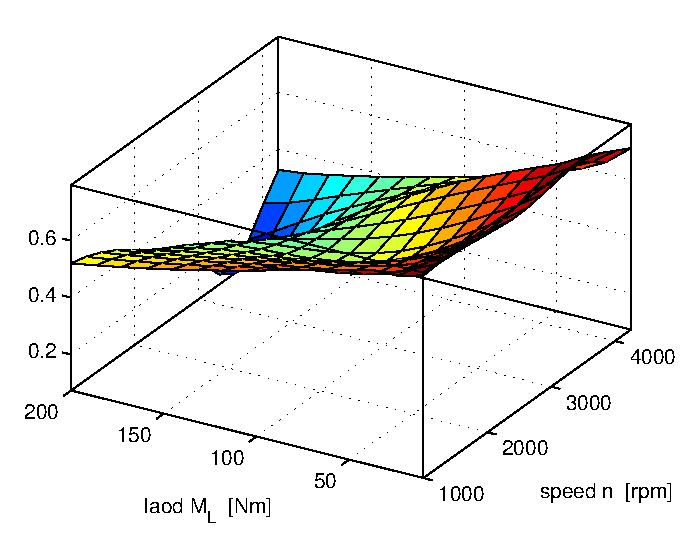
\includegraphics[width=0.75\textwidth]{img/k_surf.eps}
   \caption{Example of a figure.}
   \label{img:k_surf}
\end{figure}
\end{verbatim}

\begin{figure}[ht]
   \centering
   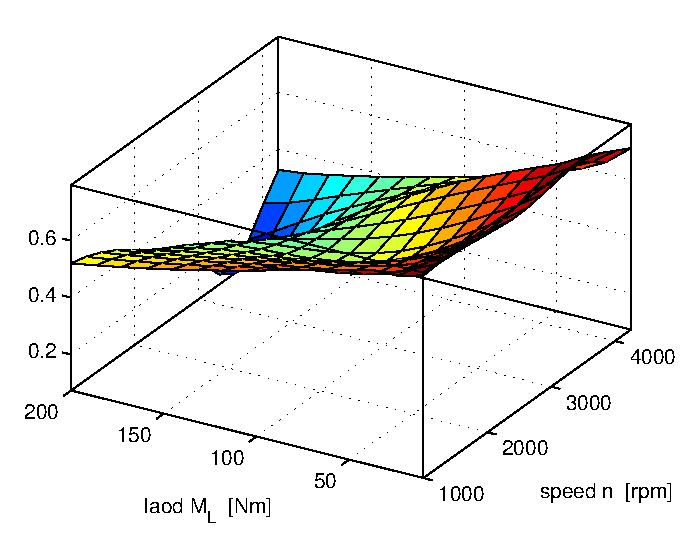
\includegraphics[width=0.75\textwidth]{img/k_surf.eps}
   \caption{Example of a figure.}
   \label{img:k_surf}
\end{figure}

Two figures are displayed next to each other using
\begin{verbatim}
\begin{figure}[ht]
  \begin{minipage}[t]{0.48\textwidth}
    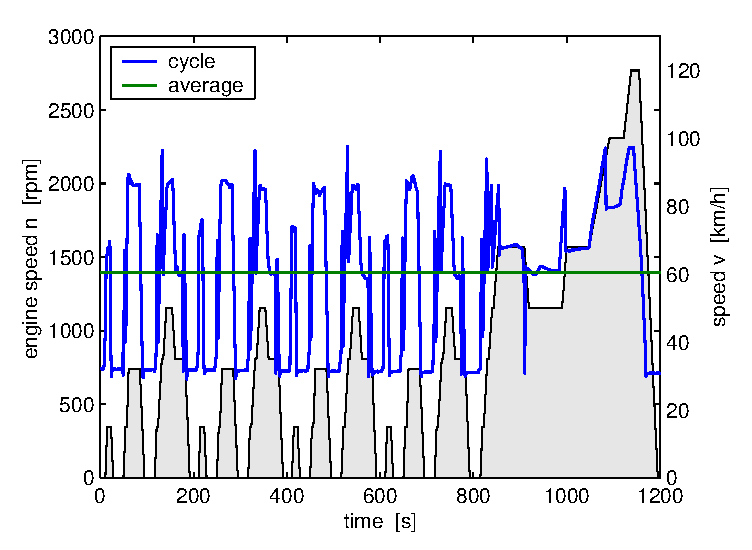
\includegraphics[width = \textwidth]{img/cycle_we.eps}
  \end{minipage}
  \hfill
  \begin{minipage}[t]{0.48\textwidth}
    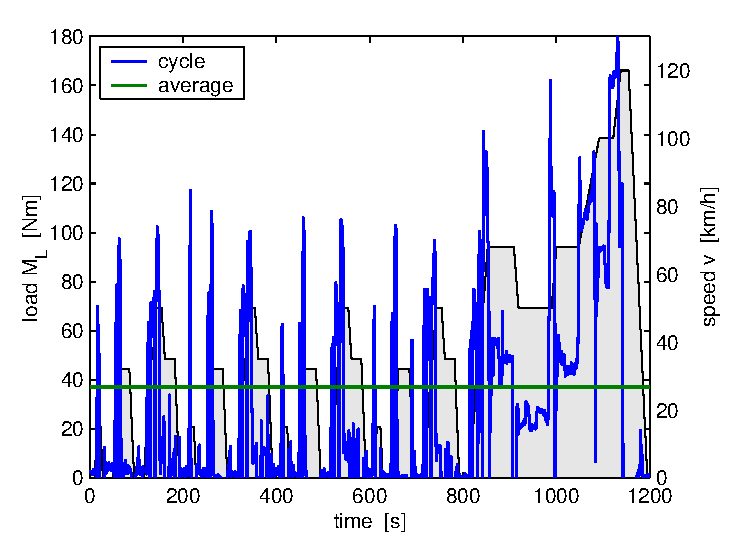
\includegraphics[width = \textwidth]{img/cycle_ml.eps}
  \end{minipage}
  \caption{Two figures next to each other.}
  \label{img:cycle}
\end{figure}
\end{verbatim}

\begin{figure}[ht]
  \begin{minipage}[t]{0.48\textwidth}
    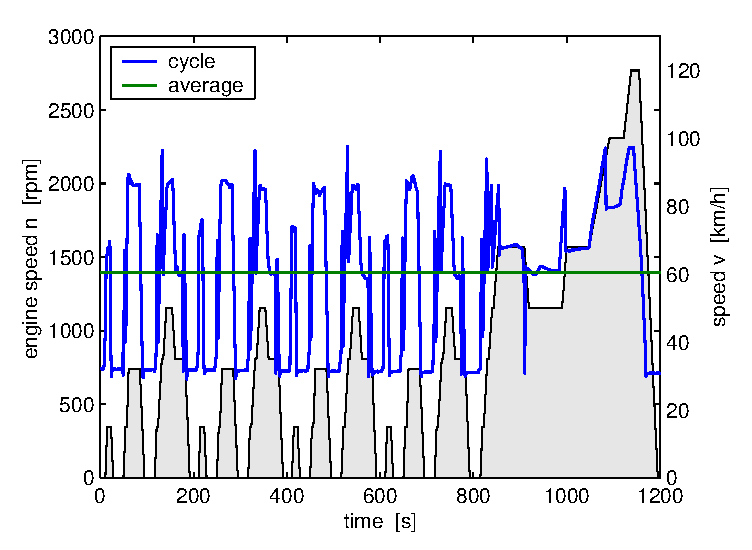
\includegraphics[width = \textwidth]{img/cycle_we.eps}
  \end{minipage}
  \hfill
  \begin{minipage}[t]{0.48\textwidth}
    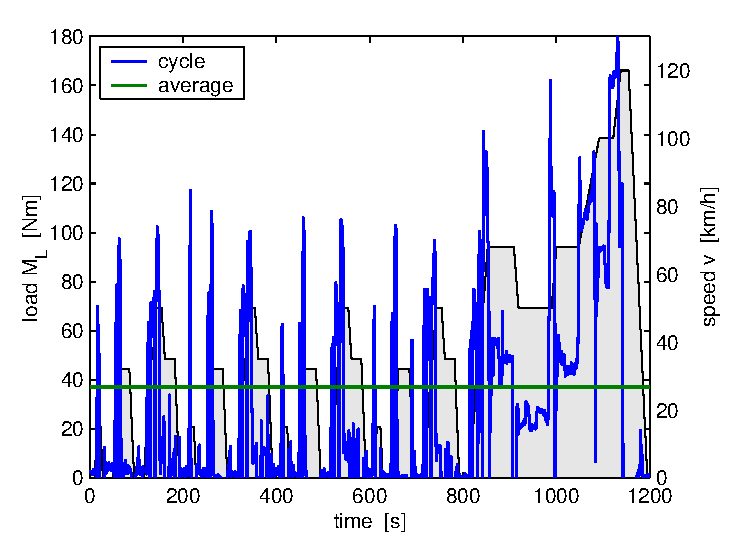
\includegraphics[width = \textwidth]{img/cycle_ml.eps}
  \end{minipage}
  \caption{Two figures next to each other.}
  \label{img:cycle}
\end{figure}

The positioning parameter \texttt{h} (here) forces your figure to be placed in the current position relative to your text. You may add \texttt{t} (top), \texttt{b} (bottom), and/or \texttt{p} (page) to allow for more flexible positioning within your document. For instance, \texttt{[tb]} forces your figure to be placed either on the top or bottom of a page.


\section{Equations}\label{sec:math}
The most common way to include equations is using the \texttt{equation} environment.
\begin{equation}\label{eq:p_me0f}
 p_\mathrm{me0f}(T_e,\omega_e) \ = \ k_1(T_e) \cdot (k_2+k_3 S^2
 \omega_e^2) \cdot \Pi_\mathrm{max} \cdot \sqrt{\frac{k_4}{B}} \, .
\end{equation}
It is recommended to use \texttt{\textbackslash mathrm\{.\}} for subscripts comprising more than two letters since it reduces the width of the subscript significantly and improves readability. The corresponding code is
\begin{verbatim}
\begin{equation}\label{eq:p_me0f}
 p_\mathrm{me0f}(T_e,\omega_e) \ = \ k_1(T_e) \cdot (k_2+k_3 S^2
 \omega_e^2) \cdot \Pi_\mathrm{max} \cdot \sqrt{\frac{k_4}{B}} \, .
\end{equation}
\end{verbatim}
Equations, such as Eq.~\eqref{eq:p_me0f}, may be referenced using \texttt{\textbackslash eqref\{.\}}. In-line mathematical content is created using \texttt{\$.\$}, for example $a^2+b^2=c^2$. It is practically possible to typeset any equation in \LaTeX. Equation~\eqref{eq:advanced} shows an example of a more advance structure.
\begin{equation}\label{eq:advanced}
x^k_n(i) = \left\{\begin{array}{ll}y(i) & \text{if}\quad x^k_{n-1}(i)\leq \mathbf{x}\\
z(i) & \text{otherwise}\end{array}\right., \text{for}\quad i=\{1,\ldots,N\}.
\end{equation}



\section{Including Code in your Document}
Include samples from your Matlab code using the \texttt{lstlistings} environment, for example
\lstset{language=Matlab,numbers=none}
\begin{lstlisting}[frame=lines]
% Evaluate y = 2x
for i = 1:length(x)

  y(i) = 2*x(i);

end
\end{lstlisting}
This example was created using
\begin{verbatim}
\lstset{language=Matlab,numbers=none}
\begin{lstlisting}[frame=lines]
% Evaluate y = 2x
for i = 1:length(x)

  y(i) = 2*x(i);

end
\end{lstlisting}
\end{verbatim}
where \texttt{\textbackslash usepackage\{mcode\}} must be included in the preamble of your document. If you want to include the entire content of a file \texttt{mycode.m} in your document, simply input the path to \texttt{mycode.m} instead of pasting the entire content into your \TeX -file
\begin{verbatim}
\lstset{language=Matlab,numbers=left}
\lstinputlisting{path/to/mycode.m}
\end{verbatim}
Including the path to your m-file also ensures that the code in your report is always up-to-date. The \texttt{\textbackslash lstset\{language=Matlab\}} command ensures that \textsc{Matlab} syntax definitions are used, but many other languages are recognised as well such as \texttt{Fortran} and \texttt{C++}.

\cleardoublepage
% \input{}
% \cleardoublepage
% \input{}
% \cleardoublepage
% ...

% Appendix______________________________________________________________________
\appendix
\chapter{Something}\label{sec:something}

Blah, blah \dots

 \cleardoublepage


\chapter{Again Something}\label{sec:again_something}

Blah, blah \dots

 \cleardoublepage



% Bibliography__________________________________________________________________
% Literature (Additional references can be added to the .bib-file manually, or by using, for example, the free application JabRef). Compile in the following order: latex -bibtex -latex -latex

\bibliographystyle{plain}
\bibliography{bibliography}

\end{document}
